% options:
% thesis=B bachelor's thesis
% thesis=M master's thesis
% czech thesis in Czech language
% english thesis in English language
% hidelinks remove colour boxes around hyperlinks

\documentclass[thesis=B,english]{FITthesis}[2012/10/20]

\usepackage[utf8]{inputenc} % LaTeX source encoded as UTF-8
% \usepackage[latin2]{inputenc} % LaTeX source encoded as ISO-8859-2
% \usepackage[cp1250]{inputenc} % LaTeX source encoded as Windows-1250

\usepackage{graphicx} %graphics files inclusion
% \usepackage{subfig} %subfigures
% \usepackage{amsmath} %advanced maths
% \usepackage{amssymb} %additional math symbols

\usepackage{dirtree} %directory tree visualisation

% % list of acronyms
% \usepackage[acronym,nonumberlist,toc,numberedsection=autolabel]{glossaries}
% \iflanguage{czech}{\renewcommand*{\acronymname}{Seznam pou{\v z}it{\' y}ch zkratek}}{}
% \makeglossaries

% % % % % % % % % % % % % % % % % % % % % % % % % % % % % % 
% EDIT THIS
% % % % % % % % % % % % % % % % % % % % % % % % % % % % % % 

\department{Department of software engineering}
\title{Specialized Information System Maintaining Patients Participating in Epileptosurgical Programme – Reporting Module}
\authorGN{Martin} %author's given name/names
\authorFN{Dvořáček} %author's surname
\author{Martin Dvořáček} %author's name without academic degrees
\authorWithDegrees{Martin Dvořáček} %author's name with academic degrees
\supervisor{Ing. Petr Ježdík Ph.D.}
\acknowledgements{This thesis has benefited greatly from the support of many people, some of whom I would sincerely like to thank here.

To begin with, I am deeply grateful for the support and guidance of Mr. Ježdík with whom I have a possibility to cooperate for past two years. Thanks to him, I could work on such an interesting topic as an implementation of an information system for a the biggest hospital in the Czech Republic.

Also, I owe special thanks to all my classmates that have somehow participated in the process of development of the GENEPI IS.

Finally, but first in my heart, my parents and my brother are due my deep gratitude for their continued moral and financial support throughout my studies, the former being of much greater importance. The broad education that I was able to enjoy while growing up has proven invaluable.
}
\abstractEN{The goal of this thesis was to implement a reporting module to GENEPI IS.
Thanks to this module it is possible to export data stored in the information system to sundry formats according to the user's choice. User may also adjust the range of exported data, according to his needs. Key requirements were robustness, reliability and security.
}
\abstractCS{Cílem této práce byla implementace reportovacího modulu do GENEPI IS.
Díky tomuto modulu je možné exportovat data uložená v informačním systému do rozličných formátů na základě výběru uživatele. Uživatel také může upravit rozsah exportovaných dat na základě svých potřeb. Mezi klíčové požadavky patřila robustnost, spolehlivost a bezpečnost.
}
\placeForDeclarationOfAuthenticity{Prague}
\keywordsCS
{
export dat, přístup na základě uživatelských rolí,
}
\keywordsEN
{
bla
}
\declarationOfAuthenticityOption{1} %select as appropriate, according to the desired license


\begin{document}

% \newacronym{CVUT}{{\v C}VUT}{{\v C}esk{\' e} vysok{\' e} u{\v c}en{\' i} technick{\' e} v Praze}
% \newacronym{FIT}{FIT}{Fakulta informa{\v c}n{\' i}ch technologi{\' i}}

\chapter{Introduction}
The reporting module, part of the GENEPI - the information system, adds an important functionality to this software. Thanks to this module the user will be able to export data saved in the system to sundry formats. This is useful for the doctors that take care of patients with epilepsy, as well as for the researchers that make analysis above the data from this system. The goal was to extend the IS with another functionality without letting the user to notice he's even using any extension. Therefore the reporting module was delicately worked into the existing source code of the GENEPI IS, using the same design patterns and approaches as the rest of the IS.

In this thesis I'll describe the design and implementation of the reporting module, as well the process of final testing of this product.

\chapter{Analysis and design}
The repoting module, as well as the whole information system, was designed given the requested robustness, accessibility, reliability and the cleanness of the source code. GENEPI has a three-tier architecture driven by Spring MVC module, uses access according to the roles of the users via Spring Security module and thanks to the optimalized data layer that uses Hibernate framework, it saves the computing resources and eases the developers to understand and extend the source code.

Due to the fact, that users, who should work with the exported data, have different levels of access and different requirements on the format of the exported data, there was a need to make the module to be able to anonymize sensitive data as well as to export data to different formats. The contracting authority also requested that the user could choose which data does he want to export.

\section{GENEPI IS}
That the reader could fully understand the functioning of the reporting module, first of all it is needed to introduce the information system that it extends. GENEPI - the information system was being created within the subjects BI-SP1 and BI-SP2 on the Czech Technical University, Faculty of Information Technologies in the school year 2012/2013 as a student's project. It should replace the original information system that was used in the Faculty Hospital Motol in Prague for maintaining patients in epileptosurgical programme. The main reasons for replacing the original information system was a fact, that it didn't comply with the current requirements of the medics, contained bugs and its design wasn't optimal. GENEPI IS is being developed in the java programming language, using frameworks Spring 4.0.2 and Hibernate 4.3.4. Front end part is realized via JSP, using HTLM5, JavaScript and CSS. Libraries that were used to ease the programming of the front end were Twitter Bootstrap 3.3.1 and jQuery 2.1.0. As a database has been chosen MySQL 5.5 and as an application server Apache Tomcat 7. All of the used software and libraries are distributed under some kind of free license. GENEPI IS is a bilingual software due to the expected deployment in the Miami Children's hospital in Florida, the United States of America. Languages that are currently supported, are czech and english, nevertheless thanks to the suitably implemented localization it is easy to extend the application and add any other language. During the whole period of the programming of the system, the team consulted the approach often  and regularly with contracting authority, to fully meet the needs of the medics.

The frameworks that were used to implement the back end are: 

\begin{enumerate}

\item{Java 7}

Java is the foundation for virtually every type of networked application and is the global standard for developing and delivering embedded and mobile applications, games, Web-based content, and enterprise software. Java is designed to enable development of portable, high-performance applications for the widest range of computing platforms possible. By making applications available across heterogeneous environments, businesses can provide more services and boost end-user productivity, communication, and collaboration—and dramatically reduce the cost of ownership of both enterprise and consumer applications.\cite{java}

\item{Apache Tomcat application server}

Apache Tomcat is an open source software implementation of the Java Servlet and JavaServer Pages technologies. Apache Tomcat is developed in an open and participatory environment and released under the Apache License version 2. Apache Tomcat powers numerous large-scale, mission-critical web applications across a diverse range of industries and organizations.\cite{apache}

\item{MySQL Community Server}

The MySQL software delivers a very fast, multi-threaded, multi-user, and robust SQL database server. MySQL Server is intended for mission-critical, heavy-load production systems as well as for embedding into mass-deployed software.\cite{mysql}

\item{Spring Framework}
The Spring Framework provides a comprehensive programming and configuration model for modern Java-based enterprise applications - on any kind of deployment platform. A key element of Spring is infrastructural support at the application level: Spring focuses on the "plumbing" of enterprise applications so that teams can focus on application-level business logic, without unnecessary ties to specific deployment environments.\cite{spring}

\item{Spring MVC}

Spring's Web MVC framework is designed around a DispatcherServlet that dispatches requests to handlers, with configurable handler mappings, view resolution, locale and theme resolution as well as support for upload files.\cite{springmvc}

\begin{figure}[ht]\centering
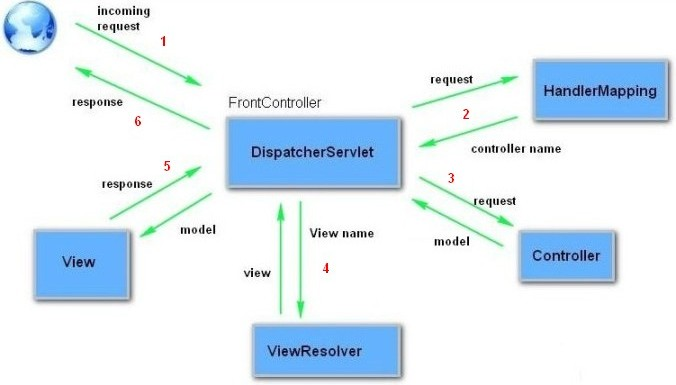
\includegraphics[width=0.5\paperwidth]{SpringMVC}
		\caption{Spring MVC web-flow}
\end{figure}

\item{Spring Security}

Spring Security is a powerful and highly customizable authentication and access-control framework. It is the de-facto standard for securing Spring-based applications.\cite{springsecurity}

\begin{figure}[ht]\centering
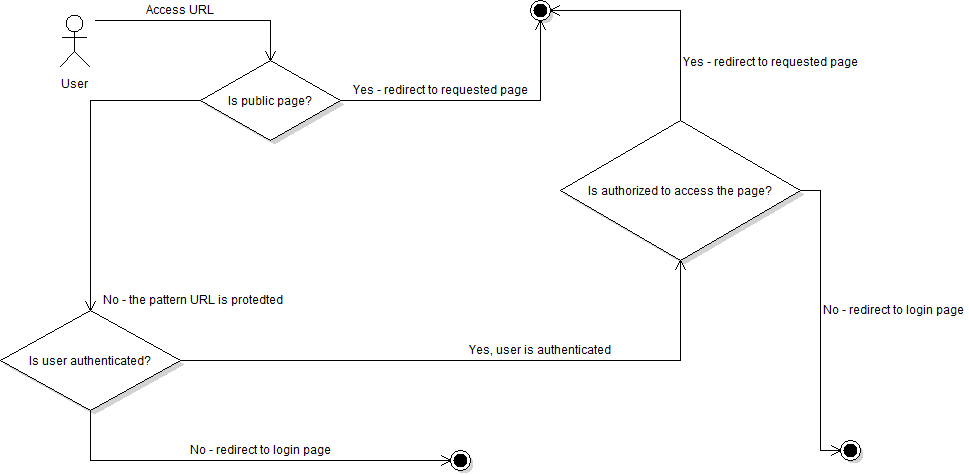
\includegraphics[width=0.5\paperwidth]{SpringSecurity}
		\caption{Authentication and Authorization flow}
\end{figure}

\item{Hibernate}

Hibernate takes care of the mapping from Java classes to database tables, and from Java data types to SQL data types. In addition, it provides data query and retrieval facilities. It can significantly reduce development time otherwise spent with manual data handling in SQL and JDBC. However, unlike many other persistence solutions, Hibernate does not hide the power of SQL from you and guarantees that your investment in relational technology and knowledge is as valid as always.\cite{hibernate}

\end{enumerate}

Used front end technologies are: 
\begin{enumerate}

\item{HTML5}

HTML5 contains powerful capabilities for Web-based applications with more powerful interaction, video support, graphics, more styling effects, and a full set of APIs. HTML5 adapts to any device, whether desktop, mobile, tablet, or television.\cite{html}

\item{JavaScript}

JavaScript (often shortened to JS) is a lightweight, interpreted, object-oriented language with first-class functions, most known as the scripting language for Web pages, but used in many non-browser environments as well such as node.js or Apache CouchDB. It is a prototype-based, multi-paradigm scripting language that is dynamic, and supports object-oriented, imperative, and functional programming styles.\cite{javascript}

\item{CSS}

Cascading Style Sheets (CSS) is a simple mechanism for adding style (e.g., fonts, colors, spacing) to Web documents.\cite{css}

\item{JSP}

JavaServer Pages (JSP) technology enables Web developers and designers to rapidly develop and easily maintain, information-rich, dynamic Web pages that leverage existing business systems. As part of the Java technology family, JSP technology enables rapid development of Web-based applications that are platform independent. JSP technology separates the user interface from content generation, enabling designers to change the overall page layout without altering the underlying dynamic content.\cite{jsp}

\item{Twitter Bootstrap}

Twitter Bootstrap is the most popular front-end framework for developing responsive, mobile first projects on the web. \cite{bootstrap}. It is build with HTML, CSS and JavaScript. Thanks to this framework it was much easier to create responsive front end with pleasant and ergonomic look and feel.

\item{jQuery}

jQuery is a fast, small, and feature-rich JavaScript library. It makes things like HTML document traversal and manipulation, event handling, animation, and Ajax much simpler with an easy-to-use API that works across a multitude of browsers. With a combination of versatility and extensibility, jQuery has changed the way that millions of people write JavaScript.\cite{jQuery}

\end{enumerate}



\section{Design of the reporting module}
Architecture of the reporting module doesn't differ from the architecture of the rest of the information system. Thanks to this, I could guarantee the robustness and the security of this module. It has also provided me an easy and elegant way to access the other components in the system.

In this tree diagram you may see the parts of the IS, that concern the reporting module:

	\dirtree{%
		.1 Backend.
		.2 src.
		.3 main.
		.4 java\DTcomment{java classes}.
		.5 cz.
		.6 cvut.
		.7 fit.
		.8 GENEPI.
		.9 businessLayer.
		.10 service\DTcomment{interface of the services}.
		.10 serviceImpl\DTcomment{implementation of services}.
		.10 VO\DTcomment{view objects}.
		.9 dataLayer.
		.10 DAO\DTcomment{interface of the DAO}.
		.10 DAOImpl\DTcomment{implementation of DAO}.
		.10 entity\DTcomment{entities}.		
		.9 presentationLayer\DTcomment{controllers}.
		.4 resources\DTcomment{property files}.
		.4 webapp\DTcomment{files for front-end}.
		.5 resources\DTcomment{front-end libraries, pictures and other media}.
		.5 WEB-INF.
		.6 tags\DTcomment{templates for jsp}.
		.6 views\DTcomment{jsp files}.
	}


\subsection{Design of the back end part}
Back end part of the reporting module was designed to follow the three-tier architecture of the rest of the system. Thus the classes that this modul uses, are devided into three different packages. Every package contains classes that belong to the same tier. These packages are called Presentation layer, Business layer and Data layer. 

\subsubsection{Presentation layer}
In the presentation layer there is a controller - a Spring MVC component that calls function according to the HTML request and its URL that is mapped to a particular function. This function executes simple operations such as verification of passed parameters and calls to the other layers. The results of the functions from other layers may be saved to a org.springframework.ui.Model object and passed to front end. This layer never executes any more complicated actions, as those should be done within the Business layer nor doesn't access the database as this should be done within the Data layer. Functions of a controller usually return the name of a view - a .jsp file - that should be displayed to a user.
\subsubsection{Business layer}
There are three packages in in this tier - concretly those are service, serviceImpl and VO. 

Service contains interfaces whereas serviceImpl contains classes that implement those interfaces from service package. It is analogical as in the data tier which I will describe in great details in the next paragraph.

In serviceImpl classes there is usally implemented some more complicated logic, that shouldn't be implemented within Presentation layer, like adjusting of VOs, sorting of lists of objects under some conditions and many other actions.

The third package - VO - contains classes, that are used to transform classes from a form in which the data come from the database - in the enitity classes - to a form, that is more propriate for work within Business tier.
\subsubsection{Data layer}
This layer contains three packages - DAO, DAOImpl and entity. In the DAO package, there are interfaces of the data access objects, in DAOImpl are the classes that implement the interfaces from DAO package and finally in entity package, we can find the entity classes.

In DAOImpl classes you can find the functions, that are used to access the database and to get some data from it. There is a direct use of hibernate functions or queries in HQL.

In entity classes is described, how the structures of the tables in the database look like. Every entity contains a property for every single column of the table. The type of this variable must match the type of the column of the table. If these conditions wouldn't be satisfied, the database query would fail and the AS would throw out org.hibernate.MappingException`.

Every property has to have a getter and a setter as well. Thanks to anotations from javax.* and org.hibernate.validator.constrains.* it is possible to check the requirements for attributes of the input that should be saved to the database, ie. minimal or maximal size, regexp pattern or if the input may be blank or NULL.

Mandatory is also a hibernate anotation @Column, as it describes the mapping of the property to the certain table in the database.

I would like to point out the generic GenericDAO and GenericDAOImpl classes that have been implemented.
These are abstract classes that were implemented to ease the process of programming of the other DAO and DAOImpl classes.

In the GenericDAOImpl class there are implemented the most used methods, that may be used by any entity such as save, delete, getCount, getCountOfUnhidden, findByID and many other. The GenericDAO class is interface of GenericDAOImpl class, as in the usall in the rest of the project.

The other DAO and DAOImpl methods extend these generic classes so then it wasn't needed to implement these basic functions to every single class and the programmer had to programme only those functions, that were unique for that certain class.

\subsection{Design of the front end part}
As well as the beck end part, the front end had to follow the style and design of the rest of the system. If I wouldn't do so, the work with reporting module could be confusing for users. On the basis of these facts, it was needed to implement frontend based on the same technologies as the rest of the GENEPI IS. Thanks to this approach the UX from work with this module is positive and user accepts reporting module as a casual part of the IS.

\chapter{Realisation}
All that will be described in this chapter is located in the business layer. The standard approach when performing an export is following:
\begin{enumerate}
\item{ The user chooses in the export view the properties that he wants to include to the exported file, the format, anonymization option and hits the export button }
\item{ PatientExportPOST method in PatientController class is called and according to the given parameters is calls method to export the data to the right format. It also checks if the data should be anonymized and if the user isn't authorized to see sensitive data, then it sets the anonymize flag to true automatically. All given parameters with all those informations are passed to called export function in the Bussines tier.}
\item{ In this step we've moved from Presentation tier to Business tier, where one of the methods for export to certain format was called. This is the part, where the data is being written to the file itself. The program iterates through all the patients that user wanted to export and gradually prints out their data.}
At first the patient's header is printed out. This header contains information about patient such as his age, gender, age at the beginning of the epilepsy and other important data. It may also contain sensitive data such as his name, address or other contact information.
\item{ In the last step is the user redirected to an URL of the newly created file with exported data to download. This file persists on the server and can be repeatedly downloaded. The time that is this file accessable depends on the setting of the server CRON, as this should regulary delete old files in the directory dedicated for export files.}

\end{enumerate}

\begin{figure}[ht]\centering
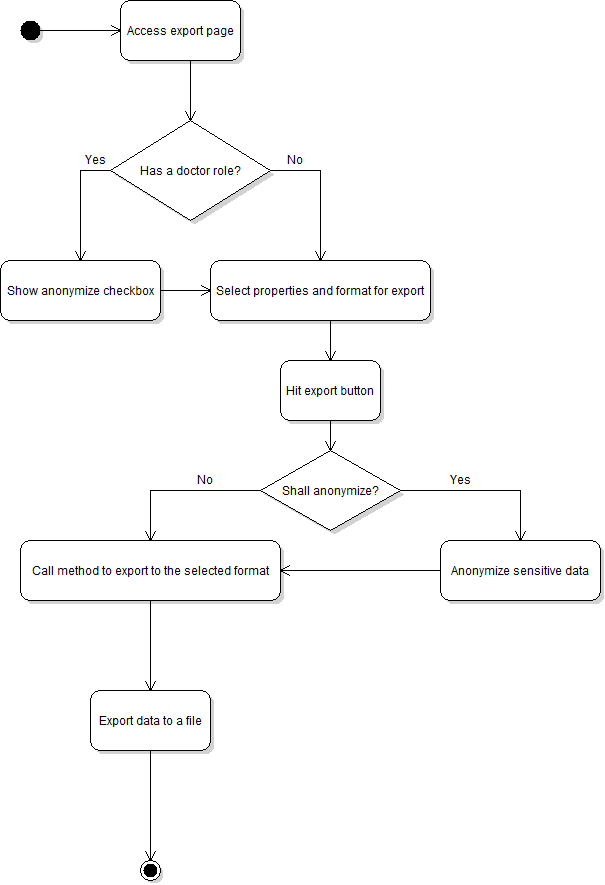
\includegraphics[width=0.6\paperwidth]{exportDiagram}
		\caption{export activity diagram}
\end{figure}

The goal was to make the whole process secure, reliable and easy to understand for programmer who would read the code, as well as for the user that would use the reporting module. Thanks to the chosen design and implementation approach, were these requirements satisfied.
\section{Customization of the export}
There was a strong demand from the contracting authority to create a module that would let the user to customize the report. Every patient can have filled in fifteen cards. This means circa 340 properties that can be stored for every single patient. Nevertheless not all of them are needed to be exported in certain situations. Therefore was needed to implement some solution, that would allow user to select only those cards or properties of those cards, that should be exported.
Due to a high amount of those properties, it was quite challenging to create solution, that would meet the requirements and will be user-friendly at the same time. I've chosen treeview on the front end and special entity on the back end.

On the front end there was implemented a customized treeview, where every item has a checkbox. Patient's cards are represented by the nodes, whereas porperties of these cards can be represented by the leaves of this tree or nodes as well. They may be nodes, if they denote some category that can hold some properties that couldn't exist withou their parent category. By checking and unchecking these items, the user can choose, what all should be involved in the exported data. When unchecking the node, also all leaves of this node are deselected. On the other hand, by selecting even a single leaf from an unselected branch, the parent node is selected as well.
Here I attach a simple example of the treeview I was writting about:


\begin{figure}[ht]
	\dirtree{%
		.1 Anamnesis\DTcomment{anamnesis card}.
		.2 Anamnesis property.
		.2 Another anamnesis property.
		.1 Seizures\DTcomment{seizure card}.
		.2 Seizure property.
		.2 Another seizure property.
		.1 ....
		.1 ....
		.1 Neuropsychology\DTcomment{neuropsychology card}.
		.2 Neuropsychology inner node.
		.3 Neuropsychology property.
		.3 Another Neuropsychology property.
		.2 Another Neuropsycholgy inner node.
		.3 Neuropsychology property.
		.2 Neuropsychology property.
		.1 ....
		.1 ....
		.1 Outcome\DTcomment{outcome card}.
	}
\end{figure}

After confirming the export form, the state of the treeview is saved to an instance of an entity called ExportParams. This entity has a boolean property for every single value from the treeview in the export form. Thanks to this, I am able to determine, which properties the user wanted to export and which didn't. It gives me another advantage - I can save the current setting of the treeview for a later usage, but I will write about this feature later.

\section{Export to the particular formats}
During the  programming of the classes that procure the logic of the reporting, I was trying to use the fact, that there already exist java libraries that can export data to docx, pdf, xls and csv formats. I also avoided the duplication of the code by transforming data from one format to another. Thanks to these measures, it is much easier to do changes in the code of the classes that handle export itself and it also eases the understanding of the code for anybody, who would read it.
\subsection{txt}
Export to the text format is realized by components form java.io.* package. Specifically java.io.FileOutputStream, java.io.OutputStreamWriter and as last java.io.BufferedWriter. Output is encoded to the UTF-8 format. Every property is printed out to a new line, sections are delimited by dash lines, star lines or empty lines.
\subsection{docx}
Export to the docx format was not as easy as to the txt, so I decided to look up suitable libraries, compare them and use that one, that would best suit my needs. After researching the possible solutions I ended up with two libraries - Apache POI and docx4j.

I've chosen to use docx4j because it has provided me more functionalities and clearer API then Apachi POI could. The main problem I had with Apachi POI was the formating of the cells, when I wanted to to format data to the tables. I could hardly adjust the size of the cells and redefine my own styles of headers and text. Docx4j provided me a really easy and elegant way to solve these issues.
\subsection{xls}
As well as for the docx format, I used the fact that there already were programmed libraries for export to xls.
I've chosen to use Apache POI library, as this library provides me anything I could need to export data to an xls file, such as merged cells, creating of new lists and changing the background color of the cells.
\subsection{pdf}
There are of course java libraries that provide you some way to export data to pdf format as well, nevertheless I've chosen different approach. While I already had implemented the export to docx, I've chosen not to implement export to pdf, but to create file with data exported to docx and using the classes form apache.poi.xwpf.converter.* package convert this file to pdf. Thanks to this approach I didn't duplicate the code because the only logic needed to format and print out the data for export was already implemented in the export to docx. After transforming docx file to pdf, the original docx file is deleted and only the newly created pdf file persists.
\subsection{csv}
Before I started to implement the export to csv format, I was also thinking, if I should implement whole logic of export to csv, but then I decided to proceed similarly as in the case of implementation of the export to pdf. Nevertheless in this case I don't use file with data exported to docx, but file created by export to xls, as this format can be easily transformed to csv and vice versa. During the export to csv I create at first an xls file with exported data and then I walk through this file and print out the values to the file via the classes from java.io.* package. These are the same classes, that have been used in the export to txt. Based on the requirements of the contracting authority, the comma, as a standard delimiter in csv format, has been replaced with semicolon. The main reason of this change was a fact, that every card, that patient may have, contains comment, which is a text, which may also contain commas. As the semicolon is a much less used character in the sentences, it was decided to use it as a delimiter. Otherwise the report could look confusingly for the user.
\section{Security and anonymization}
In GENEPI IS there are 5 main levels of an access, according to the visibility of the patient's data.
\begin{figure}[ht]
	\begin{enumerate}
	\item{Users}
	
	User role is a basic role that every new user gets from the system by default. This role allows you to acces the homepage 	and your user profile. Without any further role, the user is not allowed to perform any further actions.

	\item{Administrators}

	Administrators don't have any access to the patient's data. They are not even able to access the URL to view or export 			these data. They're the only users who may create new users a edit user's roles. They may also edit user's details and change passwords.
	\item{Researchers}

	Researchers have limited access to patient's data - they are not allowed to see sensitive data. Nevertheless they are 			still able to see lists of users, with limited options use advanced search and anonymized export data. Researchers are 			not allowed to modify patients's data.
	\item{Doctors}

	Doctors have full access to patient's data, they are allowed add new patients and modify their data. Nevertheless after every change, the patient is set as unverified. This means, that those changes weren't checked by an authorized person, can't be with certainty trusted and shouldn't be included to any research. Doctors by default doesn't have authority to verify patients whose data were changed and are set as unverified.

	\item{Superdoctors}

	Users with role Superdoctor have the same priviledges as users with role Doctor. Moreover they have the right to verify 		unverified patients.

	\end{enumerate}
\end{figure}

Because of this fact, it was needed to implement some way, how to anonymize the exported data. To reporting module I have implemented two types of anonymization - optional and manadatory.

Optional anonymization is accessable for doctors and superdoctors only. Before they commit the export, they can decide if they want to anonymize the exported data. This could be usefull for example in situations, when the doctor needs to provide the data to somebody, who normally doesn't have an access to the system and can't see the sensitive informations at the same time. On the other hand, the doctor still has a possibility to export unanonymized data, which might be usefull for the medical purposes.

Mandatory anonymization is done automatically, when somebody, who doesn't have sufficient access level, wants to export data. This feature will prevent anybody unauthorized from seeing the sensitive data of the patients. Anonymized data will be mostly used by researchers, who make analysis upon the data and don't need to know the names and addresses of patients, because they can distinguish them according to their IDs, which is a mandatory property that is printed out for every patient in every export.
\section{Custom configurations}
Customization of the configuration of exported data, was one of the key features of this module. Due to the fact, that there are several types of users who work with this IS, it's needed to count with that, that the ways how they need to use it differs. Researchers usually do some analysis above some part of the data from the IS, whereas doctors usally need some more complex report about patient's health state and the process of the treatment.

It is obivous, that settings of these configurations will be needed regulary, as it is not expected that users would need to create unique configuration for every single export he'd like to perform. Because of this, it was decided that users should have an option to save their adjusted configuration for a later use. Reporting module for GENEPI IS distinguishes two types of saved configurations.

First of them is configuration saved by a user with the Superdoctor role. This configuration may be set as generic. That means that the user chose to let his configuration to propagate through the system, so other users may see and use it.

The other type are user's private configurations. Every user with sufficient access level to access the export view is allowed to create and use them. These are configurations that were created by a user himself and are available for him only. The other users are not able to use these configurations, nor to see them.

Deleting of configurations is possible as well. Private configurations can be deleted by a user that can see them in his list of private configurations list and not by anybody else. 

On the other hand generic configurations are visible to all users in the system, therefore it is needed to determine, if a user who wants to delete some generic configuration, has even the right to perform this action. To delete a generic configuration, the user has to own a Superdoctor role. Then he's allowed to delete any generic configuration created by any other user. If user doens't have the Superdoctor role, then the delete button for generic configurations is not even displayed to this user in the export view.
On the following pictures you can see the activity diagram of saving and then deleting of a configuration from the point of view of the user.
\begin{figure}[ht]\centering
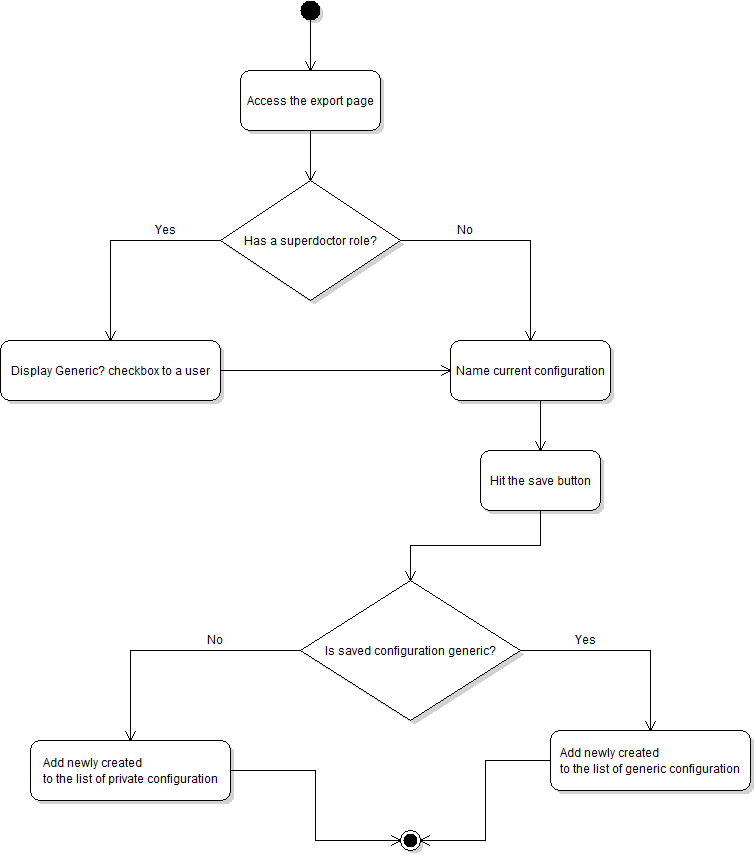
\includegraphics[width=0.5\paperwidth]{createConfigurationDiagram}
		\caption{Create configuration activity diagram}
\end{figure}

\begin{figure}[ht]\centering
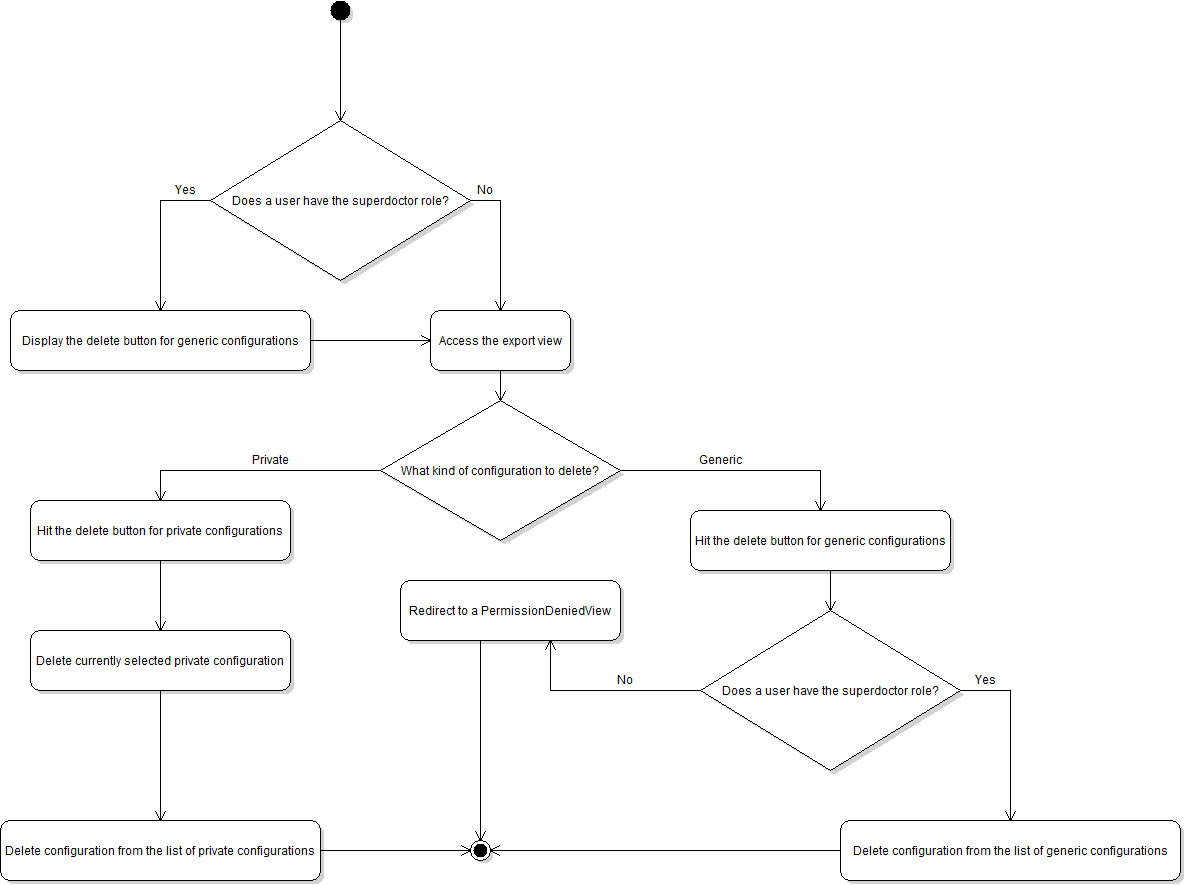
\includegraphics[width=0.5\paperwidth]{deleteConfigurationDiagram}
		\caption{Delete configuration activity diagram}
\end{figure}



\section{Graphical user interface of the reporting module}
On the following pictures I'll explain all components, that are used to controll the export view. During the phase of design and implementation of the view, I had to take into account the fact, that users of this module need a user-friendly interface that could provide them all tools that they could need to customize exports.

On the first picture, you can see the interface for loading and deleting of custom configurations. In the first row, there is a combobox with generic custom configurations which the user may load or even delete, if he's a creator of this configuration.

\begin{figure}[ht]\centering
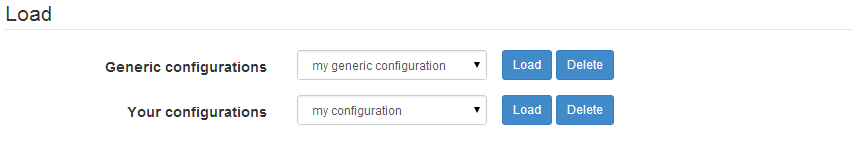
\includegraphics[width=0.5\paperwidth]{load}
		\caption{Loading and deleting of a custom configuration}
\end{figure}

On the next picture there is displayed a section for export itself. Firstly there is a list of IDs of patients that are prepared for an export. The user may access the patient's overview by clicking his ID. Next it's needed to choose the format for export via several radiobuttons. In the case, that user chooses as a format docx or pdf, a checkbox appears and lets him to choose if exported data should be formated into tables or as a text. If the user has the Doctor role assigned, then he's able to see a combobox, that allows him to let to anonymize exported data.

\begin{figure}[ht]\centering
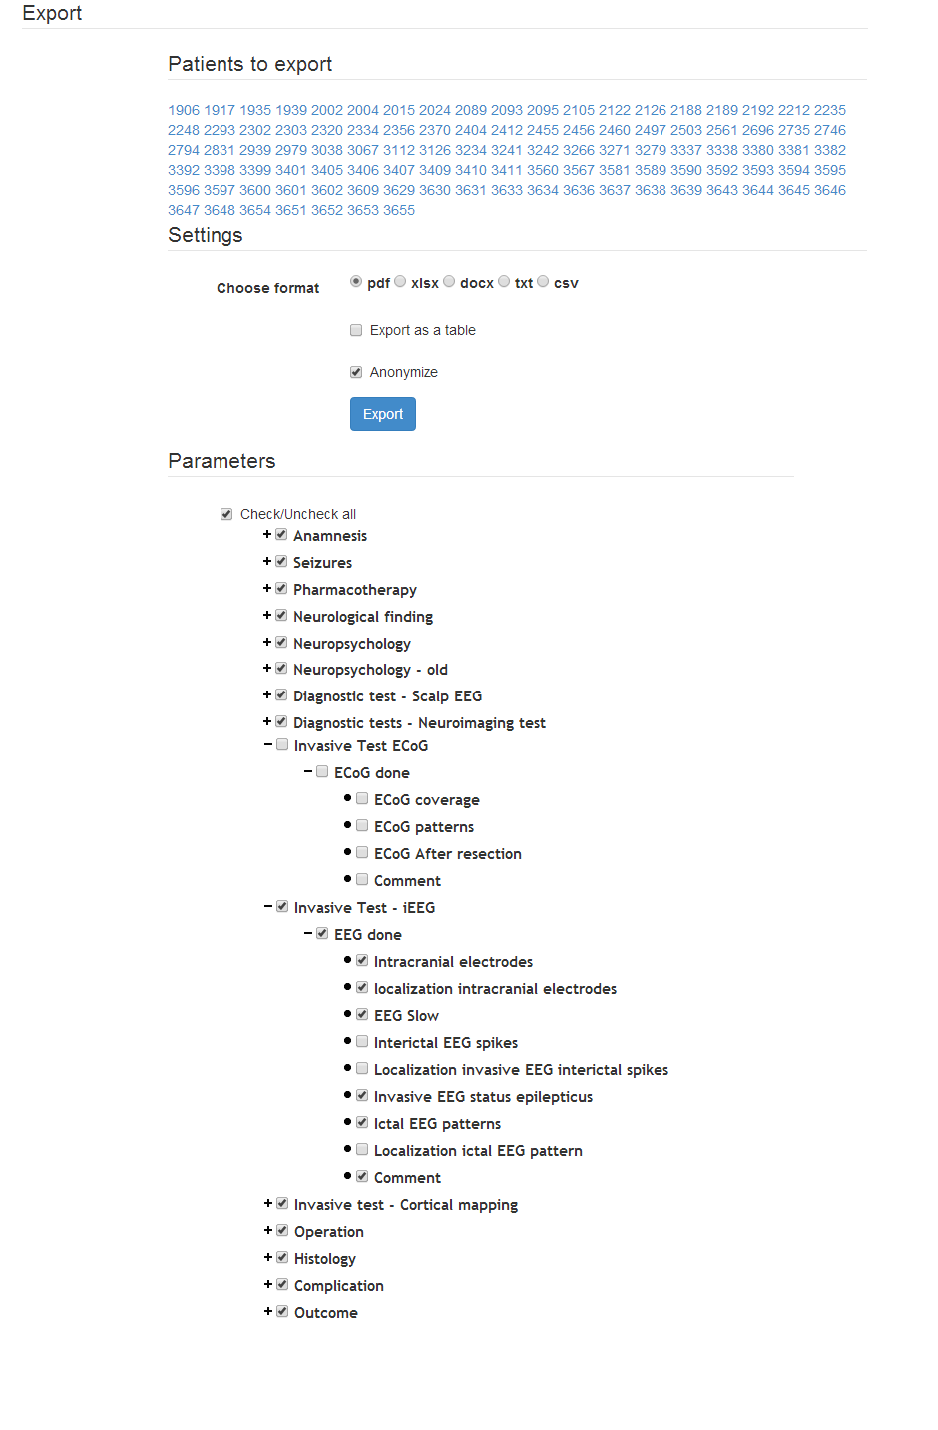
\includegraphics[width=0.6\paperwidth]{export}
		\caption{Selection of format and customization of an export}
\end{figure}

On the last picture you can see the interface for saving custom configurations. There is a textfield for naming the configuration and if the user has the Superdoctor role, then he may check the checkbox to make the configuration generic.


\begin{figure}[ht]\centering

\includegraphics[width=0.5\paperwidth]{save}
		\caption{Saving of a custom configuration}
\end{figure}

\chapter{Testing}

Testing of the reporting module as well as the GENEPI IS itself was being performed during the development by the developers themselves and by a member of the team who held the position of a tester. After key  functionalities were implemented, Ing. Ježdík Ph.D got the access to the system and tested it on usual use cases. He of course had many change requests that could enbetter the application or found bugs that should be fixed. Nowadays the GENEPI IS with reporting module should be deployed on produciton servers in the Faculty Hospital Motol and fully replace the existing applicaiton. As in the most of the cases from commercial sector, it is awaited, that users will also have some change requests. But those are expected to be minor change requests, mostly on a front end and should be implemented within a few MD.

As a source code repository was chosen GitHub. Thanks to this, it was easy to collaborate on a development on GENEPI IS, as well as to see the changes in the source code or to revert the changes to previous versions of the code. You may find the GENEPI's public GitHub repository on the URL \verb| https://github.com/Dworzaaa/database-epileptic-patients|.

During the development there was Jenkins CI deployed on the development server. In a nutshell Jenkins CI is the leading open-source continuous integration server. Built with Java, it provides 922 plugins to support building and testing virtually any project. \cite{jenkins}. I find this tool very useful as it was regulary downloading the whole application from the GitHub repository, building it and deploying to our development server, that Mr. Ježdík kindly provided us. Thanks to this, the process making any new changes, features or fixes and following process of testing them, become really smooth and literally a matter of one click. Jenkins CI is also used to perform automatized test before every deployment to make sure that newly added features didn't have any bad influence on the rest of the existing code.

\begin{conclusion}
The goal of my bachelor's thesis was to design and implement a reporting module for GENEPI IS. This extension should be robust, reliable, secure with user-friendly GUI.

I've created a tool greatly extends the possibilities, that GENEPI IS could provide to doctors and researchers, who would use it. Without the reporting module, GENEPI IS would be only a tool to store and look up informations about patients. But now it become a tool, that can provide to users structured and customized reports. Those reports may be used as a source of important informations about the patient's health state and about the process of his treatment during the surgery as well as the source of data for analysis and researches.

Thanks to the possibility to customize exports, the doctors can select to export only those data, that are important for given medical intervention. As it is expected that the set of requested informations to given interventions will not change frequently, the doctors can also use the feature of the module to configure the export once, then save the configuration, and then just load it anytime they would need it, without any need of further configuration.

Another possibility of using the reporting module are analysis made by researchers. Researchers shouldn't usually be allowed to see sensitive data about patients. Thus there comes in handy the feature of automatical anonymazation of the patient's data. Also a possibility to export unlimited count of patients during one export to one file is usefull, because researchers need larger amount of data to make any analysis. Exporting every single patient to separated file one by one, would be really user-unfriendly solution. It is also awaited, that researchers will use diffirent formats than doctors. Whereas doctors are awaited to use mostly docx or pdf format, researchers will probably use xls, csv or txt. These formats can be easily parsed and processed to other software for further analysis.

These all were the reasons why in the end it is possible to execute export to 14 sundry formats. Those are 5 basic formats, 5 more in anonymized variant. Docx and pdf export can be also formated to tables. With anonymized variant we get 4 more formats. This should be sufficient solution to meet the needs of any user of GENEPI IS.

To sum up I must say, that I'm really satisfied with the software I've created on the basis of the requests of the doctors from the Faculty Hospital Motol in Prague. I belive that it will serve doctors and researchers well and make their work and research much easier. This all should lead to ZLEPSENI the treatment of the patients with epilepsy.

I feel really proud, that result of my bachelor's thesis will be deployed in the biggest hospital in the Czech Republic and will be there used to help real patients. I also belive that that my work will have its share on helping the mankind to understand such as insidious disease which epilepsy is and maybe even to save somebody's life.

\end{conclusion}

\bibliographystyle{csn690}
\bibliography{mybibliographyfile}

\appendix

\chapter{Acronyms}
% \printglossaries
\begin{description}
	\item[AS] Application Server
	\item[CI] Continuous Integration
	\item[DAO] Data Access Object
	\item[GUI] Graphical User Interface
	\item[HQL] Hibernate Query Language
	\item[IS] Information System
	\item[JSP] JavaServer Page
	\item[MD] Manday
	\item[MVC] Model View Controller
	\item[XML] Extensible Markup Language
	\item[VO] View Object
\end{description}

\chapter{Contents of enclosed CD}
To my bachelors thesis I enclose a CD, that contains all important data, that are needed to start your own Apache Tomcat AS, MySQL database and depoloy GENEPI IS. It also contains source codes of GENEPI IS and libraries that it uses. In the Database directory is also enclosed model for MySQL Workbench, where the reader may see the structure of the database. In the same folder you can also find migration scripts. These are important when migrating from the information system that was previously used in the Faculty Hospital Motol to GENEPI IS. Migration scripts allow you to copy data from previously used database to the databse that is being used by the GENEPI IS.
Thanks to this, the reader should be able to administrate or even modify GENEPI IS without any larger problems. If the reader would like to use enclosed Apache Tomcat AS and/or MySQL database, he has to agree and follow the licence agreements that are enclosed in the same directories as the software, that is being distributed under them.

Next important directory is the directory with samples of exported data. This folder contains 14 files with all possible formates of exported data - pdf, docx, xls, csv, txt - all of these formates in both anonymized and unanonymized variants and both printed to as a plain text and formated to a table for pdf and docx.

The reader may also find useful directory that contains deployment packages of the results of the previously mentioned projects from the subjects BI-SP1 and BI-SP2. The documentation to these projects is included in that directory.

Another content of enclosed CD is text directory, that contains this this theis in pdf and ps format and readme.txt file, where is in great deatails described the content of the CD.

\begin{figure}
	\dirtree{%
		.1 readme.txt\DTcomment{the file with CD contents description}.
		.1 Apache Tomcat\DTcomment{the directory that contains Apache Tomcat}.
		.1 Database\DTcomment{the directory that contains MySQL databse and database scripts}.
		.2 MySQL\DTcomment{the directory that contains MySQL database}.
		.2 data\DTcomment{the directory that holds model of the database and migration scripts}.
		.1 war\DTcomment{the directory with war file}.
		.1 Backend\DTcomment{the directory of a maven project}.
		.2 src\DTcomment{the directory of GENEPI IS source codes}.
		.3 main.
		.4 java.
		.5 cz.
		.6 cvut.
		.7 fit.
		.8 GENEPI\DTcomment{the directory of source code of an implementation}.
		.4 resources\DTcomment{the directory configuration files}.
		.4 webapp.
		.5 resources\DTcomment{the directory of librarires for front end}.
		.6 WEB-IF.
		.7 spring\DTcomment{the directory for spring context file}.
		.7 tags\DTcomment{the directory of templates for jsp pages}.
		.7 views\DTcomment{the directory of jsp pages}.
		.3 test\DTcomment{the directory of source codes of unit tests }.
		.1 Previous projects\DTcomment{the direcotry of results of BI-SP1 and BI-SP2}.
		.2 BI-SP1\DTcomment{the directory of the BI-SP1 project}.
		.2 BI-SP2\DTcomment{the direcotry of the BI-SP2 project}.
		.1 Sample Data\DTcomment{the directory that contains samples of exported data}.
		.1 Text\DTcomment{the thesis text directory}.
		.2 thesis.pdf\DTcomment{the thesis text in PDF format}.
		.2 thesis.ps\DTcomment{the thesis text in PS format}.
	}
\end{figure}

\end{document}
